\documentclass{article}
\usepackage[a4paper, total={6in, 8in}]{geometry}
\usepackage{graphicx}
\usepackage{hyperref}
\graphicspath{ {./temp/} }

\usepackage[utf8]{inputenc}

\title{CMSC 6950 Final Project - pymagicc}
\author{Behnam Farhadi}
\date{June 2021}

\begin{document}
\maketitle

\section{Introduction}
Pymagicc\cite{Gieseke2018} is a Python interface for the Fortran-based reduced-complexity climate carbon cycle model MAGICC (Meinshausen, Raper, and Wigley 2011). Aiming at broadening the user base of MAGICC1, Pymagicc provides a wrapper around the MAGICC binary, which runs on Windows and has been published under a Creative Commons Attribution. NonCommercial-ShareAlike 3.0 Unported License. Pymagicc itself is licensed under the GNU Affero General Public License v3.0.

\section{Tasks}
This project utilises the Pymagicc module to achieve the below computational tasks and visualizations.

\subsection{ Task 1- Generate Radiative Forcing|Greenhouse Gases vs year}
In this task, we read data from RCP26, RCP45, RCP60, RCP,85 scenario files, convert the data in
MAGICData format to a pandas DataFrame, and then build visualizations to show Radiative 
Forcing|Greenhouse Gases for RCP26, RCP45, RCP60 and RCP 85 scenarios based on each 
year. 
\begin{figure}[h]
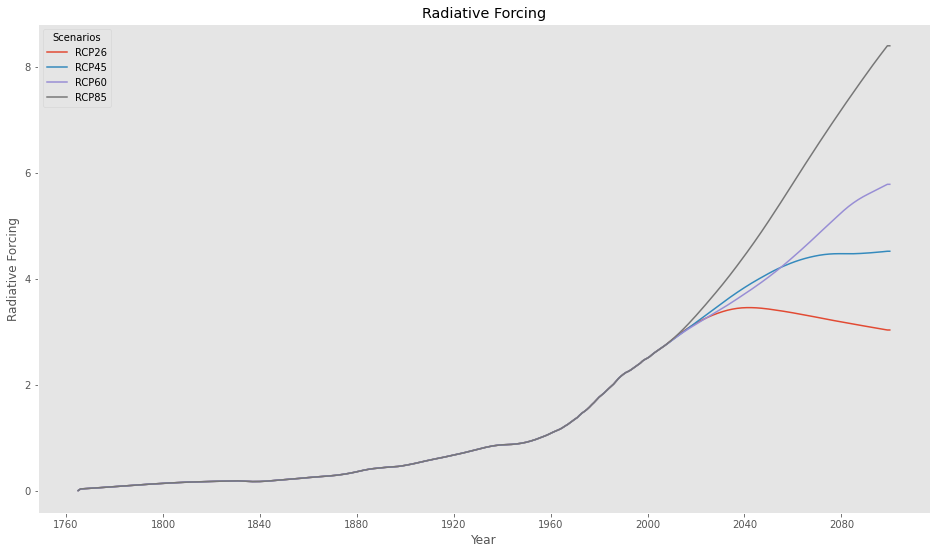
\includegraphics[width=\textwidth,height=\textheight,keepaspectratio]{Radioactive.png}
\end{figure}

\clearpage
\subsection{Task 2- Generate Emissions|CO2|MAGICC AFOLU vs Year}
In this task, we run the MAGICC model on RCP26, RCP45, RCP60 and RCP85 scenarios and
visualize the Emissions|CO2|MAGICC AFOLU projections for each of the given projections from
1765 to 2100.
\begin{figure}[h]
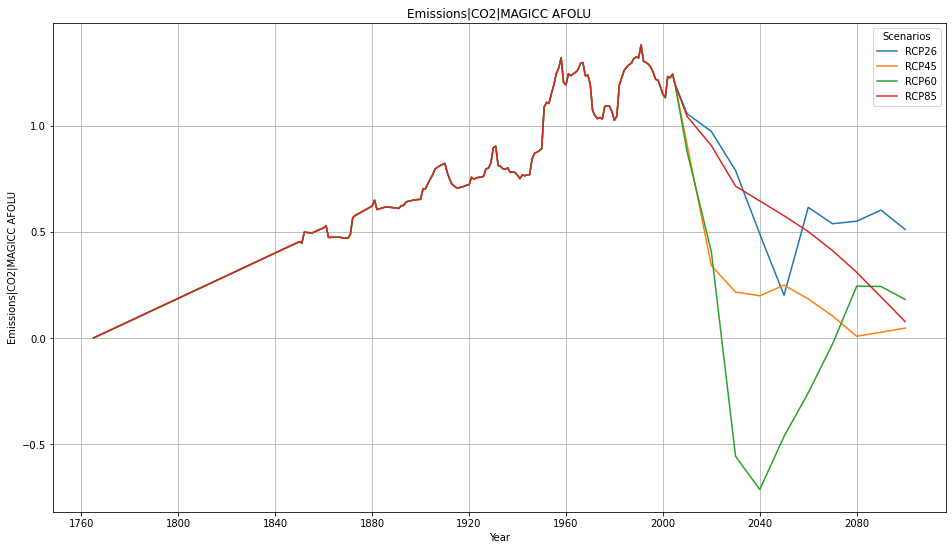
\includegraphics[width=\textwidth,height=\textheight,keepaspectratio]{Emmissions.png}
\end{figure}
\section{Install}
First,we have to download the Miniforge3-Linux-x86\_64 from below link:\\
\href{https://github.com/conda-forge/miniforge/releases/latest/download/Miniforge3-Linux-x86_64.sh}https://github.com/conda-forge/miniforge/releases/latest/download/Miniforge3-Linux-x86\_64.sh\\
Then, we install it by this command: bash Miniforge3-Linux-x86\_64.sh  and then:\\
conda install matplotlib pandas seaborn notebook pymagicc\\
then:\\
sudo apt-get update \\
and:sudo dpkg --add-architecture i386\\
 last:\\
 sudo apt-get install wine
 Our environment for run pymagicc is ready know.\\
\begin{thebibliography}{9}
\bibitem{latexcompanion} 
Robert Gieseke, Sven N. Willner, and Matthias Mengel. Pymagicc: A python wrapper for the
simple climate model magicc. Journal of Open Source Software, 3(22):516, 2018.
\end{thebibliography}
\end{document}